\typeout{ ====================================================================}
\typeout{ this is file main.tex, created at 20 Nov 2012                       }
\typeout{ maintained by Gustavo Rabello dos Anjos                             }
\typeout{ e-mail: gustavo.rabello@gmail.com                                   }
\typeout{ ====================================================================}

\documentclass[a4paper,fleqn,12pt,twoside]{report} % tipo de folha e documento
\usepackage[T1]{fontenc}              % acentuacao e hifenizacao portuguesa
%\usepackage[utf8]{inputenc}
\usepackage[brazil]{babel}            % pacote de linguagens 
\usepackage{indentfirst}              % tab na primeira linha do paragrafo 
\usepackage[hmargin=30mm,vmargin=25mm]{geometry}
\usepackage[pdftex]{graphicx}         % pacote para inclusao de figuras,
\usepackage{subfig,wrapfig}           % pacote para figuras duplas (subfigure)
\usepackage{amssymb,amsmath,amsfonts} % pacote matematicos
\usepackage{multirow}                 % multiplas linhas por coluna
\usepackage{pictexwd,color}			  % ambiente para PICTEX
\usepackage{tocbibind}				  % para inclusao de bib e ind na TOC
\usepackage{alltt,verbatim,moreverb}  % para entrada verbatim comandos LaTeX
\usepackage{rotating}				  % para rotacionar alguns flutuantes
\usepackage{amscd}					  % para setas longas

\graphicspath{{./figuras/}{./figs/}}  % onde encontrar as figuras...

\renewcommand{\baselinestretch}{1.5}  % espacamento entre linhas 
\setlength{\mathindent}{15mm}         % espacamento das equacoes

%%%%%%%%%%%%%%%%%%%%%%%%%%%%%%%%  MATH MACROS %%%%%%%%%%%%%%%%%%%%%%%%%%%%%%%%
\newcommand{\tr}{{\,\rm tr}\,}
\newcommand{\sen}{{\,\rm sen}\,}
\newcommand{\senh}{{\,\rm senh}\,}
\newcommand{\diverg}{{\,\rm div}\,}
\newcommand{\grad}{\,\mathbf{grad}\,}
\newcommand{\rot}{\,\mathbf{rot}\,}
\newcommand{\uvet}{\mathbf{u}}
\newcommand{\vvet}{\mathbf{v}}
\newcommand{\cvet}{\mathbf{c}}
\newcommand{\wvet}{\mathbf{w}}
\newcommand{\xvet}{\mathbf{x}}
\newcommand{\gvet}{\mathbf{g}}
\newcommand{\fvet}{\mathbf{f}}
\newcommand{\nvet}{\mathbf{n}}
\newcommand{\tvet}{\mathbf{t}}
\newcommand{\Imat}{\mathbf{I}}
\newcommand{\Eo}{\mathrm{Eo}}
\newcommand{\N}{\mathrm{N}}
\newcommand{\Mo}{\mathrm{Mo}}
\newcommand{\ca}{\cellcolor[gray]{0.5}}
\newcommand{\cb}{\cellcolor[gray]{0.0}}
%%%%%%%%%%%%%%%%%%%%%%%%%%%%%%%%%  -- END -- %%%%%%%%%%%%%%%%%%%%%%%%%%%%%%%%%

%%%%%%%%%%%%%%%%%%%%%%%%%%%%%%% MACROS PORTUGUES %%%%%%%%%%%%%%%%%%%%%%%%%%%%%%
\newcommand{\ih}{\'\i}
\newcommand{\ao}{\~ao }
\newcommand{\oes}{\~oes }
\newcommand{\cao}{\c c\~ao }
\newcommand{\coes}{\c c\~oes }
\newcommand{\aon}{\~ao}
\newcommand{\oesn}{\~oes}
\newcommand{\caon}{\c c\~ao}
\newcommand{\coesn}{\c c\~oes}
%%%%%%%%%%%%%%%%%%%%%%%%%%%%%%% MACROS PORTUGUES %%%%%%%%%%%%%%%%%%%%%%%%%%%%%%

\begin{document}
 
\chapter{Introdu\c c\~ao aos Escoamentos Bif\'asicos}

A proposta deste cap\'itulo \'e dar ao leitor uma vis\~ao geral dos
m\'etodos mais importantes encontrados na literatura de escoamentos
bif\'asicos. Uma revis\~ao  bibliogr\'afica \'e tamb\'em inclu\'ida para
ajudar o aluno a encontrar as principais refer\^encias e nomes de
autores que desenvolveram metodologias para a investiga\cao deste
importante fen\^omeno.

\subsection{Introdu\c c\~ao}

O conceito de fase, atrav\'es dos princ\'ipios de termodin\^amica
cl\'assica, \'e descrito como o estado macrosc\'opico da mat\'eria no
qual sua estrutura f\'isica e em sua composi\cao qu\'imica s\~ao
homog\^eneas. Na presen\c ca de duas ou mais fases, origina-se o que
chamamos de escoamentos multif\'asicos, onde o termo bif\'asico se
refere \`a presen\c ca de apenas 2 fases (Ex. bolha de ar em um copo de
\'agua). 


\subsection{Equa\c c\~oes de Governo}

Em escoamentos bif\'asicos, as equa\c c\~oes que modelam o fen\^omeno
f\'isico s�o as mesmas que modelam escoamentos monof\'asico, por\'em o
termo de tens\~ao superficial \'e acrescentado ao lado direto da
equa\cao de conserva\cao de quantidade de movimento (referencia para
capitulo do Pontes). Uma vez que a dedu\cao das equa\c c\~oes de
conserva\cao para escoamentos monof\'asicos se encontra no volume 1
deste livro, tomamos a liberdade de apresentar estas equa\c c\~oes,
aplicadas a escoamentos bif\'asicos, em sua forma euleriana vetorial, 
para o modelo de um fluido (one-fluid).

\begin{equation}
	\rho \bigg[ \ 
	\frac{\partial \rho v_x}{\partial x}+
	\frac{\partial \rho v_y}{\partial y}+
 	\frac{\partial \rho v_z}{\partial z}
	\bigg]
	=
	\rho \nabla \cdot \vvet 
	=
	0
\label{eq:cm9}
\end{equation}

Desde que $\rho \ne 0$ em todas as fases, a equa\cao de conserva\cao de
massa \'e apresentada como:

\begin{equation}
	\nabla \cdot \vvet = 0
\label{eq:cmFinal}
\end{equation}

Aqui, $\vvet$ representa o vetor de velocidades que para o caso
bidimensional contem as componentes $x$ e $y$ e no caso tridimensional
$x$, $y$ e $z$. Como mencionado anteriormente, a equa\cao de conseva\cao
de quantidade de momento \'e modificada com a adi\cao do termo de
tens\~ao superficial $\fvet_{s}$, resultando em:

\begin{equation}
	\rho \bigg [ \frac{\partial \vvet}{\partial t} + 
	\vvet \cdot \nabla \vvet \bigg ]
	= -\nabla p + \nabla \cdot [ \mu (\nabla \vvet + \nabla \vvet^T) ] + 
	\rho \gvet +
	\fvet_{s}
\label{eq:qm16}
\end{equation} \vspace{0.0cm}

Na equa\cao acima, $\rho$ e $\mu$ representam densidade e viscosidade
respectivamente. No entanto, no modelo de um fluido (one-fluid), estes
valores permanecem constantes em cada fase, por\'em n\~ao s\~ao
necessariamente constantes em todo o espa\c co.  $t$ representa a
vari\'avel temporal, $p$ o campo de press\~ao e $\gvet$ o campo
gravitacional. 

Esta equa\cao pode ser reescrita em sua forma \emph{Lagrangiana},
tomando como base a movimenta\cao do referencial de acordo com a
movimenta\cao do fluido.

\begin{equation}
	\rho \frac{D \vvet}{D t}
	= -\nabla p + \nabla \cdot [ \mu (\nabla \vvet + \nabla \vvet^T) ] +  
	\rho \gvet +
	\fvet
\label{eq:qmFinal}
\end{equation} \vspace{0.0cm}

Neste caso, a nota\cao do lado esquerdo da equa\cao \ref{eq:qm16} \'e
compactado atrav\'es do operador derivada substantiva $D/Dt$. A
diferen\c ca dos referenciais \emph{Euleriano} e \emph{Lagrangiano} \'e
que no primeiro o referencial se encontra fixo no espa\c co, enquanto
que no segundo o referencial movimenta com a velocidade do fluido. Estes
dois referenciais ainda podem ser descritos em uma forma \'unica e
generalizada, conhecida como referencial \emph{Euleriano-Lagrangiano}
arbitr\'ario onde a referencial pode n\~ao estar nem fixo, nem
movimentando conforme o escoamento, e sim em uma velocidade
arbitr\'aria. Entretanto, a defini\cao deste referencial n\~ao est\'a
presente no escopo deste cap\'itulo. Para o leitor interessado,
recomenda-se: \cite{hughes1981} e \cite{donea1982}.

\subsection{Abordagem Num\'erica}

Em escoamentos bif\'asicos, ou \emph{two-phase flows} em ingl\^es, a
modelagem discreta da interface \'e o par\^ametro mais importante para
se obter precis\~ao nos c\'alculos. Encontra-se na literatura duas
abordagens cl\'assicas para representa\cao da interface entre dois
fluids: \emph{Euleriana} e \emph{Lagrangiana}. Estas duas abordagens
est\~ao fortemente ligadas \`a representa\cao do escoamento. Figura~(\ref{fig:interface}) representa um esquema bidimensional das
descri\c c\~oes de interface nos dois modos acima citados. 

Na descri\cao \emph{Euleriana}, tamb\'em conhecida do ingl\^es
\emph{inteface capturing}, a interface n\~ao \'e representada
explicitamente atrav\'es de objetos computacionais (n\'os, segmentos e
elementos), ao contr\'ario ela \'e definida atrav\'es de uma fun\cao de
identifica\cao de fases e deslocada atrav\'es de uma equa\cao
hiperb\'olica. Devido a sua discretiza\cao, tal equa\cao \'e uma fonte
de difusao num\'erica e deve ser tratada com aten\cao. Neste tipo de
representa\cao de interface, mudan\c cas topol\'ogicas na interface,
como coalescencia e ruptura, s\~ao facilmente modeladas. No entanto, a
descri\cao de todas as escalas presentes no problema f\'isico requer um
n\'umero de pontos computacionais mais elevado.

Na descri\cao \emph{Lagrangiana}, a interface que separa as duas fases
\'e representada atrav\'es de um conjunto de objetos computacionais,
tais como: n\'os, segmentos e elementos. Figura~(\ref{fig:interface}b)
ilustra um caso bidimensional onde a interface est\'a representada por
tais objetos como parte do dom\'inio num\'erico. Como pode ser visto, a
interface n\~ao divide nenhum elemento, com isso nenhum tratamento
especial \'e necess\'ario para modelar fortes diferen\c cas de
propriedades f\'iscias como viscosidade e densidade. Adicionalmente \`a
esta abordagem, a interface \'e representada sem qualquer difus\~ao, ou
seja, esta \'e definida com espessura zero, assemelhando-se \`a uma fiel
representa\cao da realidade. O movimento da interface \'e feito
atrav\'es do pr\'oprio campo de velocidade, sem o aux\'ilio de qualquer
equa\cao adicional. 


\begin{figure}[ht!]
		\subfloat[]{\label{fig:interface1}
		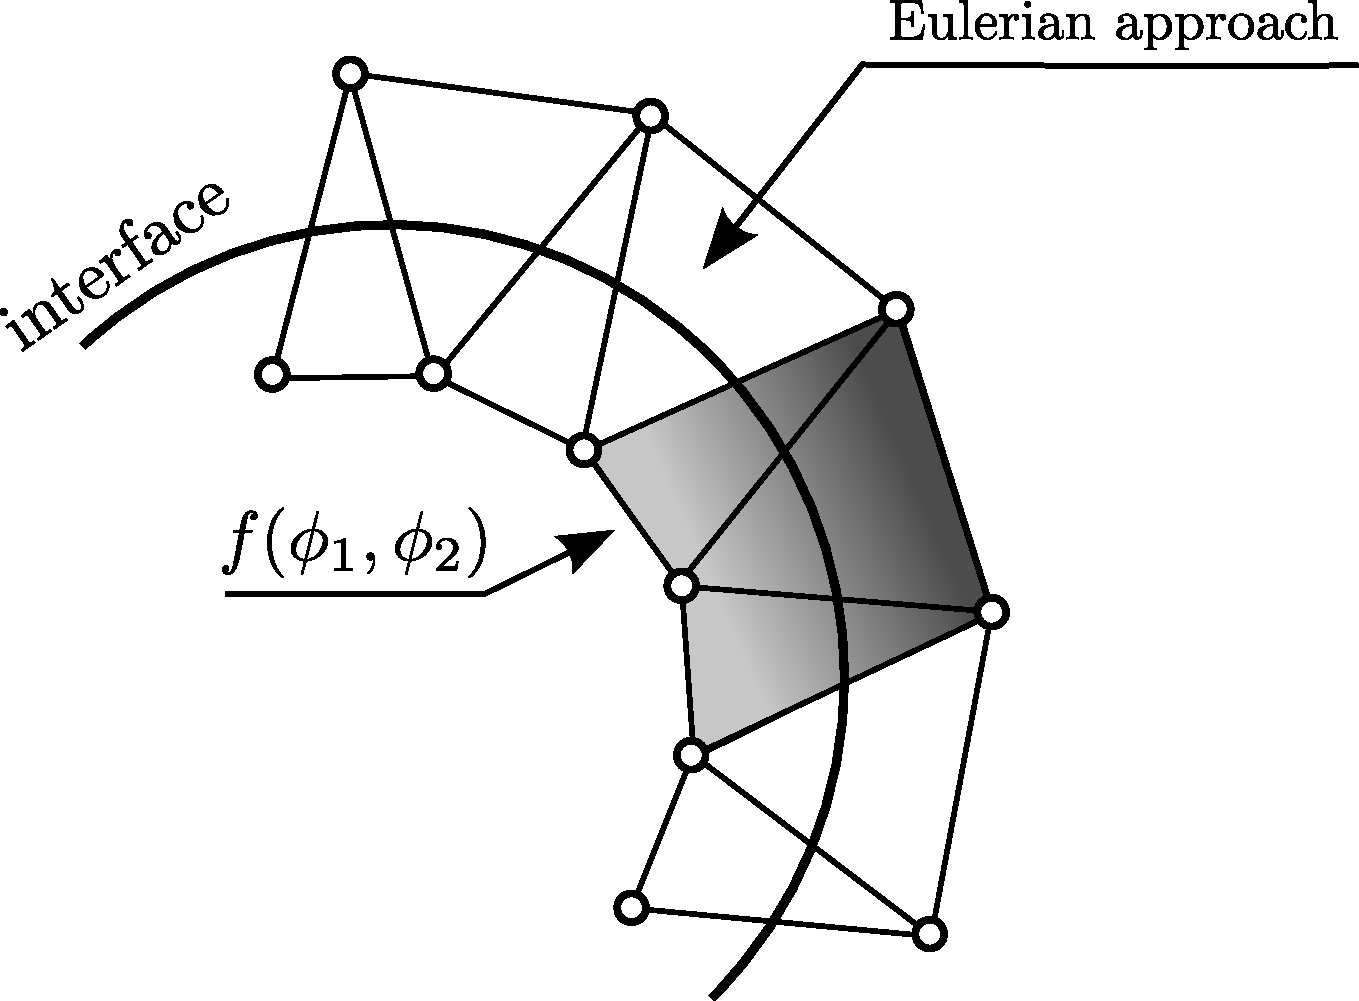
\includegraphics[scale=0.32]{interface1.pdf}}
		\subfloat[]{\label{fig:interface2}
		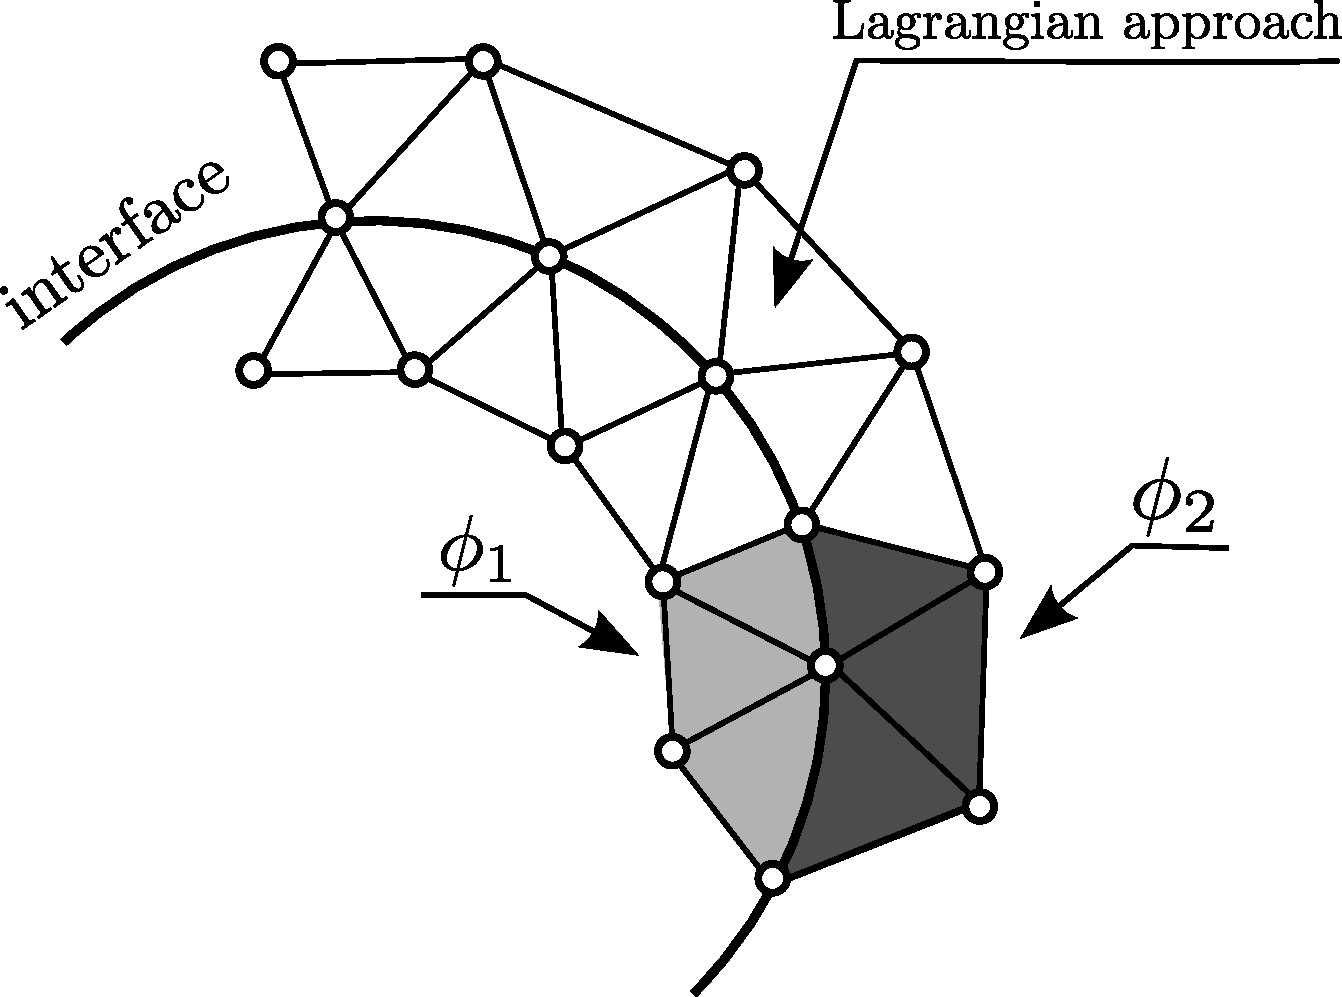
\includegraphics[scale=0.32]{interface2.pdf}}
	\caption{Representa\cao da inteface em escoamentos bif\'asicos. (a)
	Na descri\cao \emph{Euleriana}, a interface entre os fluidos \'e
	definda em uma posi\cao arbitr\'aria em rela\cao aos elementos.
	Diferentemente, (b) o descri\cao \emph{Lagrangiana} representa a
	interface atrav\'es de pontos pertencentes \`a malha computacional
	atrav\'es da defini\cao de objectos, tais quais n\'os, segmentos e
	elementos, obtendo assim uma representa\cao precisa da interface.}
	\label{fig:interface} 
\end{figure}

Entre as descri\c c\~oes \emph{Euleriana} e \emph{Lagrangiana},
diferentes t\'ecnicas est\~ao dispon\'iveis para a modelagem de
escoamentos bif\'asicos. Cada metodologia particular garante um conjunto
de caracter\'isticas com diferentes n\'iveis de programa\cao. Abaixo
ser\~ao apresentados os m\'etodos mais comumente encontrados na
literatura de escoamentos bif\'asicos.

% --------------------------------------------------------------- %
%                     Volume of Fluid - VOF                       %
% --------------------------------------------------------------- %
Em 1980, o m\'etodo volume de fluido (\emph{Volume of Fluid} ou VOF na
sigla em ingl\^es) foi proposto por \cite{hirt1981}, no qual consiste na
descri\cao de cada fase atrav\'es do volume de fluido ocupado em cada
elemento computacional. Os inteiros ``0'' e ``1'' s\~ao atribu\'idos
para definir a regi\~ao ocupada na totalidade por cada fluido e valores
intermedi\'arios s\~ao atribu\'idos nos elementos onde a interface \'e
definida. Devido \`a descontinuidade proveniente desta metodologia, uma
alta precis\ao n\~ao pode ser garantida no c\'alculo da curvatura e dos
vetores normais \`a interface. Figura~(\ref{fig:vof-interface}) mostra
um esquema bidimensional do m\'etodo \emph{VOF} em uma malha retangular
estruturada.

\begin{figure}[ht!]
		\subfloat[]{\label{fig:vof1}
		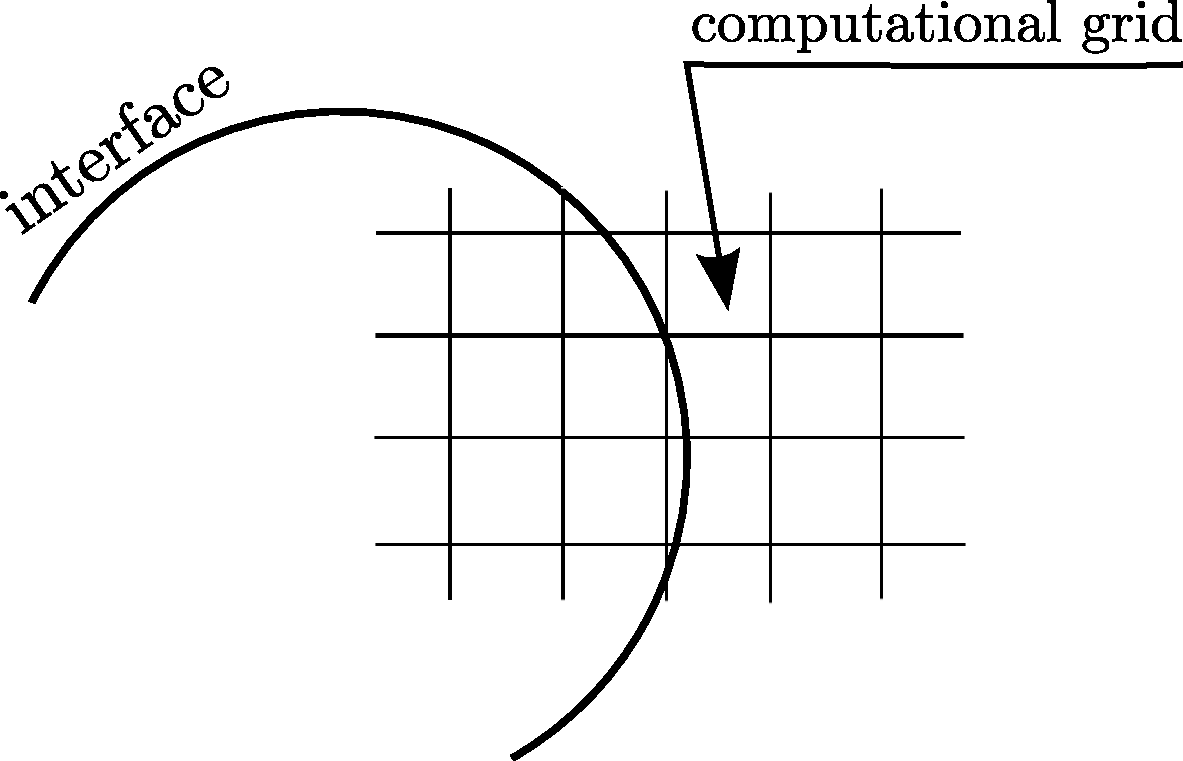
\includegraphics[scale=0.45]{vof.pdf}}
		\subfloat[]{\label{fig:vof2}
		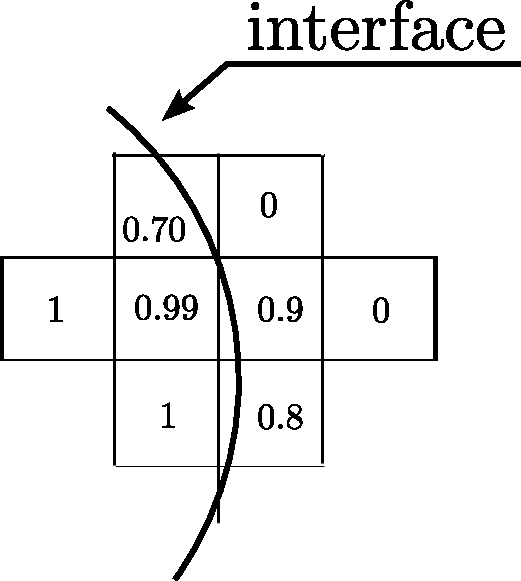
\includegraphics[scale=0.6]{vofzoom.pdf}}
	\caption{Representa\cao da interface no m\'etodo \emph{VOF}. (a) A
	interface entre os fluidos \'e definida implicitamente e localizada
	em algum lugar entre elementos computacionais. (b) A fun\cao
	\emph{VOF} \'e constru\'ida considerando-se o volume ocupado por
	cada fluido em cada elemento computacional.}
	\label{fig:vof-interface} 
\end{figure}

Um modelo bidimensional foi desenvolvido por \cite{tomiyama1993} e
depois extendido a escomanentos tridimensionais \cite{tomiyama1997}. O
c\'odigo tridimensional incluiu uma nova metodologia baseada no m\'etodo
de rastreamento de part\'iculas (\emph{particle tracking method} em
ingl\^es), na qual os efeitos de cada fase s\~ao considerados na outra
fase e vice-versa. Testes foram realizados para investiga\cao de bolha
em ascen\cao em um fluido parado. Uma grande faixa de n\'umeros
adimensionais \emph{E\"otv\"os} e \emph{Morton} foram testadas e
comparadas a resultados experimentais, com isso provando a capacidade do
c\'odigo em capturar os efeitos observados em fluidos com diferentes
propriedades. 

Em \cite{chen1998}, um modelo de escoamento bif\'asico baseado no
m\'etodo \emph{VOF} foi desenvolvido para simular escoamentos com
grande diferen\c ca na rela\cao de desidades. O modelo de for\c ca de
superf\'icie cont\'inua (continuum surface force model - CSF  em
ingl\^es) foi usado para obter-se os efeitos da tens\~ao superficial nas
equa\c c\~oes de Navier-Stokes. A coalescencia de bolhas e a bolha em
ascen\cao foram investigadas para valida\cao do c\'odigo num\'erico com
dados de literatura dispon�vies. O m\'etodo proposto apresentou boa
concord\^ancia com dados experimentais. 

Um modelo de escoamento bif\'asico bidimensional foi apresentado em 
\cite{ginzburg2000} com utiliza\cao do m\'etodo \emph{VOF} e um m\'etodo
de elementos finitos escalonado. Esta metodologia foi baseada em uma
classe de elementos facilmente encontrada no m\'etodo de elementos
finitos, chamada \emph{Crouzeix-Raviart}. Adicionalmente, um refinamento
de malha adaptativo foi utilizado para obter-se uniformidade nos
elementos de malha pr\'oximo \`a interface. Foram executados testes
est\'aticos e din\^amicos, como a bolha em ascens\~ao, encontrando-se
boas compara\c c\~oes a resultados experimentais.

Em \cite{wu1998} foi desenvolvido um modelo bidimensional e
axissim\'etrico utilizando os m\'etodo de elementos finitos para
simula\cao de escolamentos bif\'asicos atrav\'es do m\'etodo \emph{VOF}.
Um modelo modificad da for\c ca de superf\'icie cont\'inua (\emph{CSF}
foi proposto para tratar o termo de tens\~ao superficial nas equa\c
c\~oes de Navier-Stokes. Tal modelo contorna as dificuldades na
aproxima\cao da curvatura da interface e, com isso, facilita seu
c\'alculo. Resultados foram comparados com sucesso a diferentes casos
como rompimento de barragem (\emph{Dam breaking}), gota oscilante e
bolhas estacion\'arias.

% --------------------------------------------------------------- %
%                         Level-Set - LS                          %
% --------------------------------------------------------------- %
O m\'etodo de Level-Set (LS) na din\^amica de fluidos foi primeiramente
apresentado por \cite{osher1988} e se tornou uma importante ferramenta
para modelagem de escoamentos bif\'asicos. Neste m\'etodo a interface
\'e representada por uma fun\cao dist\^ancia de n\'ivel zero que \'e
movimentada pelo campo de velocidades. A curvatura e os vetores normais
\`a interface s\ao convenientemente calculados com a ajuda da mesma
fun\cao dist\^ancia, com isso uma modelagem direta da tens\~ao
superficial \'e realizada com sucesso. Apesas de sua recente apari\cao
nos modelos de escoamento bif\'asico, o
m\'etodo de Level-Set provou-se ser um dos mais importantes modelos de
din\^amicas interfaciais. Figura~(\ref{fig:ls}) mostra a representa\cao
das fun\c c\~oes dist\^ancia e Level-Set em um caso bidimensional com
dom\'inio em forma de quadrado. A fun\cao dist\^ancia \'e calculada
atrav\'es da norma 2 do espa\c co Euclidiano em cada n\'o da malha e sua
respectiva menor dist\^ancia \`a interface separando os fluidos,
matematicamente $\xvet-\xvet_I$, onde $\xvet$ \'e o n\'o da malha e 
$\xvet_I$, o n\'o mais pr\'oximo da interface. A mesma fun\cao
dist\^ancia \'e usada para o c\'alculo da fun\cao de Level-Set, que
n\~ao \'e nada mais que uma vers\~ao com sinais positivo e negativo,
representando o que est\'a em uma fase e em outra. As duas fun\c c\~oes
representam a interface quando o valor coincide com zero. 

\begin{figure}[ht!]
		\subfloat[]{\label{fig:distance}
		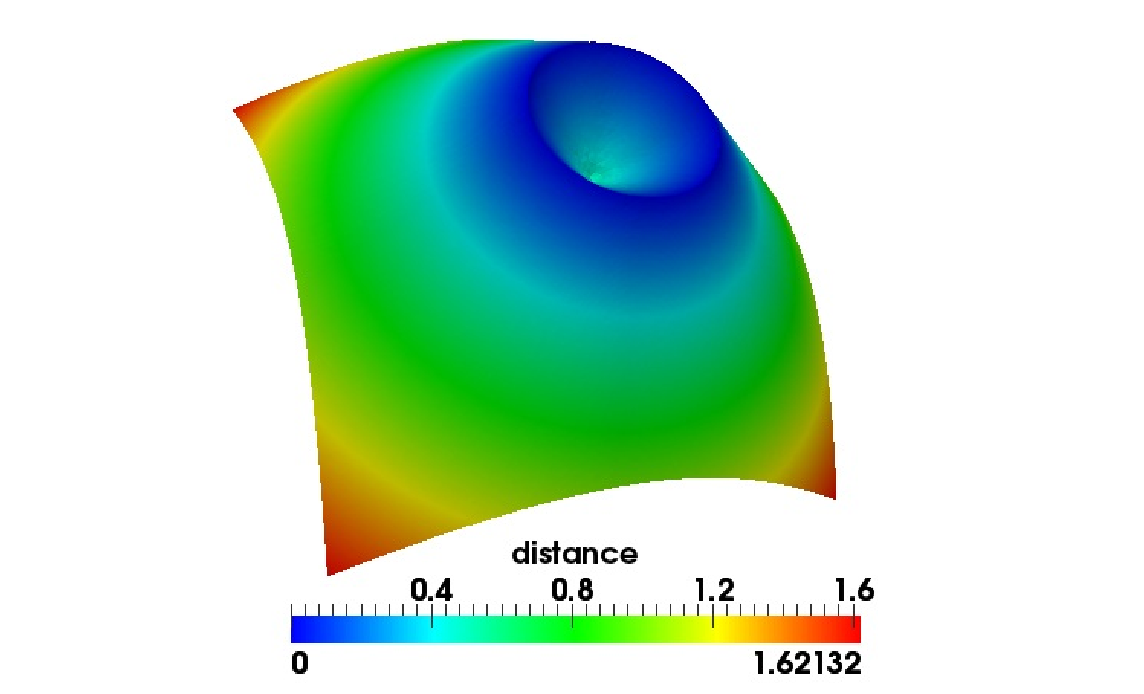
\includegraphics[scale=0.55]{distance.pdf}}
		\hspace{0.5cm}
		\subfloat[]{\label{fig:level-set}
		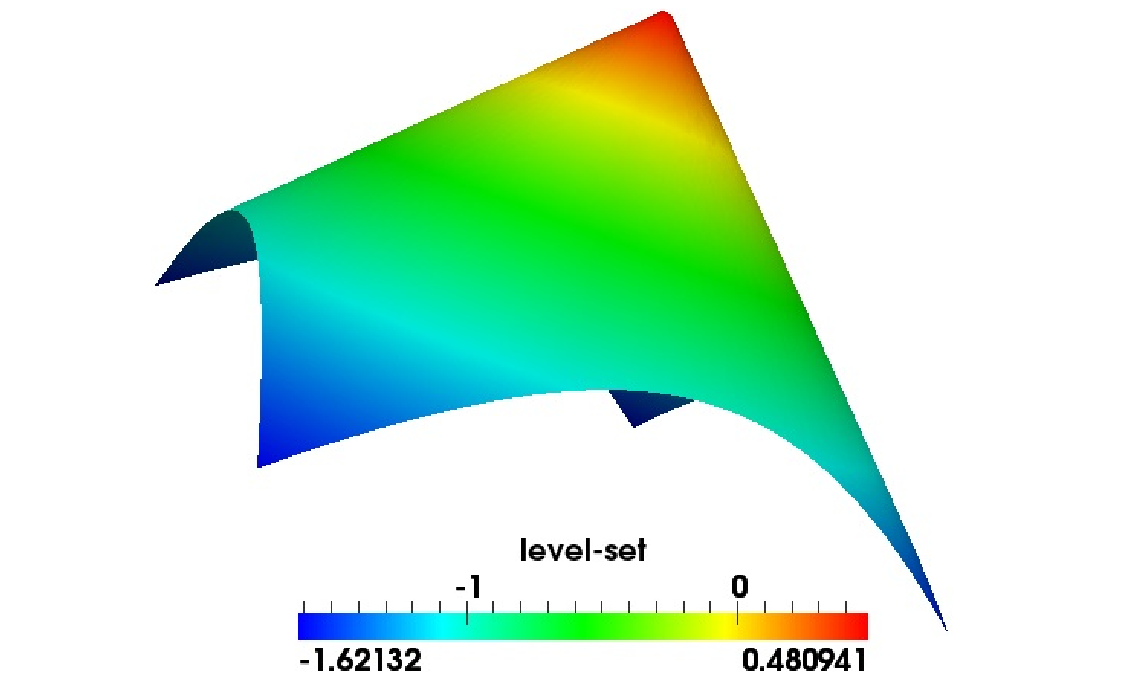
\includegraphics[scale=0.55]{level-set.pdf}}
	\caption{Representa\cao das fun\c c\~oes dist\^ancia e Level-Set. A
	interface entre os fluidos \'e localizada no meio do dom\'inio
	computacional. (a) A fun\cao dist\^ancia \'e criada atrav\'es do
	c\'alculo da dist\^ancia de cada n\'o da malha $\xvet$ para seu
	correspondente n\'o da interface mais pr\'oximo $\xvet_I$. (b) A
	fun\cao de Level-Set \'e representada como sendo a fun\cao
	dist\^ancia com sinais positivo e negativo correspondentes \`a
	localiza\cao do fluido.}
	\label{fig:ls} 
\end{figure}

O m\'etodo de Level-SEt em escoamentos bif\'asicos foi primeiramente
desenvolvido por  \cite{sussman1994} e seguido por muitos outros
autores. Eles propuseram um esquema de segunda ordem baseado em
upwind/proje\cao para o c\'alculo da solu\cao das equa\c c\~oes de
Navier-Stokes para fluidos imisc\'iveis. Foi mostrado que a conserva\cao
de mass \'e apenas garantida se a fun\cao de Level-Set \'e
reinicializada preferenciamente em todo passo de tempo. Eles realizaram
significativos testes com bolhas e gotas para valida\cao desta nova
metodologia. Adicionalemente, \cite{sussman1997} apresentaram sua
vers\~ao extendida para o caso tridimensional de superf\'icie livre.
Novamente, testes foram realizados com sucesso para valida\cao desta
nova extens\~ao atrav\'es de importantes casos, tais quais gota
est\'atica e gota oscilante em gravidade zero.

O acoplamento dos m\'etodos de Level-Set e de elementos finitos foi
apresentado por \cite{quecedo2001}, no qual as equa\c c\~oes de
escoamento de fluido foram discretizadas em uma malha triangular. Foi
proposto um m\'etodo de passo de tempo fracion\'ario no qual foi usado
para estabilizar press\~ao  e velocidade, por consequ\^encia permitindo
o uso do mesmo elemento finito para discretiza\cao  de ambas as
grandezas f\'isicas. Grandes diferen\c cas em densidade foram testadas
com sucesso e comparados a outros testes cl\'assicos na literatura.

Uma formula\cao de elementos finitos estabilizada e acoplada ao m\'etodo
de Level-Set foi desenvolvida para o c\'alculo da din\^amica de bolhas
em \cite{nagrath2005}. Um m\'etodo tipo Petrov-Galerkin foi tamb\'em
utilizado para discretizar as equa\c c\~oes de conserva\cao de
quantidade de movimento. Coalescencia e ascen\cao  de bolhas foram
estudadas e comparadas com a metodologia proposta.

Um m\'etodo num\'erico foi proposto em \cite{marchandise2006} para a
simula\cao tridimensional incompress\'ivel de escoamentos bif\'asicos. O
m\'etodo de Level-Set foi utilizado com sucesso junto ao m\'etodo de
elementos finitos estabilizado para a solu\cao das equa\c c\~oes de
Navier-Stokes. Os resultados foram ent\~ao comparados com muitos
exemplos num\'ericos comumentes encontrados na literatura, tais quais
escoamento de \emph{Poiseuille}, instabilidade de Rayleigh-Taylor,
ruptura de barragem etc. Todos os testes apresentaram boa concord\^ancia
com a literatura.

Apesar da grande utiliza\cao  do m\'etodo de Level-Set, resultados
mostraram que a implementa\cao direta deste m\'etodo ocasiona excessiva
difus\~ao num\'erica, com isso a reinicializa\cao da fun\cao de
Level-Set se faz obrigat\'oria em todo o passo tempo. Uma outra
alternativa, adotada por muitos autores, \'e o acoplamento do m\'etodo
de Level-Set com o m\'etodo VOF, formando CLSVOF (\emph{coupled
Level-Set Volume-of-Fluid em ingl\^es}). Esta nova metodologia (ver
\cite{bourlioux1995}, \cite{sussman2000} and \cite{nichita2010a}) utiliza
as principais caracter\'isticas de cada m\'etodo separado, com isso a
curvatura e os vetores normais s\~ao  calculados atrav\'es da fun\cao de
Level-Set enquanto que a interface \'e capturada a partir da fun\cao
VOF. Consequentemente, os erros de conserva\cao de massa presentes no
m\'etodo de Level-Set e o pobre c\'alculo de curvatura proveniente do
m\'etodo VOF s\~ao eliminados.

% --------------------------------------------------------------- %
% Front-tracking                                                  %
% --------------------------------------------------------------- %

Ao contr\'ario dos m\'etodos Level-Set e VOF, a descri\cao
\emph{Lagrangiana} define a interface entre fluidos explicitamente
atrav\'es de elementos computacionais. Tal descri\cao \'e conhecida como
rastreamento de interface (\emph{interface tracking} no ingl\^es).
Dentro desta classe de m\'etodos, \emph{volume-tracking} e
\emph{front-tracking} s\~ao os que mais se destacam na literatura. O
primeiro utiliza particulas marcadoras para reconstru\cao da interface,
combinando precis\~ao e rigor com relativamente baixo custo de
investimento (\cite{harlow1965},\cite{amsden1970}). O segundo,
primeiramente implementado por \cite{glimm1988}, representa a interface
atrav\'es de um conjunto de n\'os interconectados que se movem de acordo
com o escoamento calculado no referencial \emph{Euleriano}. Tal
descri\cao fornece uma representa\cao definida da interface com alta
precis\~ao, entretanto sua desvantagem est\'a na necessiade de um
tratamento explicito quando a interface apresenta mudan\c cas
topol\'oligas, como no caso de coalescence e ruptura de interface.

Em \cite{unverdi1992}, uma nova metodologia para simula\cao de
escoamentos multif\'asicos foi descrita. As equa\c c\~oes foram
discretizadas atrav\'es do m\'etodo de diferen\c cas finitas em uma
malha estacion\'aria, com a interface definida explicitamente por um
conjunto de objetos geom\'etricos tais como tri\^angulos, segmentos e
pontos. Apesar da malha computacional de fundo ser est\'atica
(descri\cao \emph{Euleriana}), a malha de interface se movia com a
velocidade proveniente do escoamento. Os vetores normais \`a interface
foram calculados a partir de fun\c c\~oes trigonom\'etricas em cada
elemento da superf\'icie e a curvatura foi calculada atrav\'es de uma
aproxima\cao da indicatrix \emph{Dupin} na superf\'icie. Por apresentar
uma descri\cao explicita da interface, tal metodologia definiu com
precis\~ao a superf\'icie que separa os fluids, entretanto as
propriedades dos fluidos n\~ao foram precisamente definidas,
necessitando ent\~ao de um tratamento num\'erico especial.  

Um modelo Level-Set \emph{Lagrangiano} foi proposto por
\cite{souza2005} para simula\cao de escoamentos incompress\'iveis 
bif\'asicos. As esqua\c c\~oes de governo foram discretizadas atrav\'es
do m\'etodo de \emph{Galerkin} e elementos finitos, enquanto que o
sistema linear resultante for tratado atrav\'es do m\'etodo da
proje\cao, visando desacoplar velocidade e press\~ao. A interface entre
fluidos era representada pela pr\'opria malha do dom\'inio e ent\~ao
movida pelo campo de velocidade. Tal modelo dispensa o uso de uma
equa\cao hiperb\'olica adicional, uma vez que a interface \'e descrita
por pontos e segmentos da pr\'opia malha computacional bidimensional. O
controle de malha foi feito atrav\'es de procedimentos padr\~oes tais
quais \emph{flipping}, adi\cao e remo\cao de arestas e n\'os. Pela
defini\cao da fun\cao de Level-Set $\phi$, foi poss\'ivel calcular
diretamente a curvatura e os vetores normais \`a interface atrav\'es das
express\~oes: $\kappa=\nabla
\cdot(\nabla \phi/|\nabla \phi|)$ e $\nvet = \nabla \phi / |\nabla
\phi|$, consecutivamente. Com isso, para satisfazer o balan\~co de
for\~ca discreto entre press\~ao e tens\~ao superficial, o gradiente da
fun\cao de \emph{Heaviside} $\nabla H$ foi usado como substituto da
fun\cao Delta de Dirac $\delta$, encontrado no modelo de for\c ca de
superf\'icie continuo (CSF). Tal abordagem \'e comumente encontrada em
modelos \emph{Eulerianos}, por\'em mostrou-se adequado para m\'etodos do
tipo \emph{Interface-tracking}, uma vez que o salto de press\~ao
atrav\'es da interface foi precisamente calculado.

O grupo da Universidade de Massachustts sugeriu um modelo completo de
malha din\^amica para simula\cao de escoamentos tipo superf\'icie livre
e bif\'asicos (\cite{perot2003},\cite{quan2006}), no qual difere da
abordagem de malha fixa. Neste caso, a discretiza\cao das equa\c c\~oes
de governo foi feita sobre uma malha n\~ao estruturada com o aux\'ilio
de um m\'etodo de passo fracional exato. Tal t\'eqnica melhora a
defini\cao da interface, uma vez que o salto de propriedades f\'isicas
\'e mantido definido. A valida\c c\~ao da metodoligia foi realizada com
sucesso atrav\'es de v\'arios testes num\'ericos comparativos, mostrando
que a t\'ecnica pode ser utilizada para modelagem de escoamentos
bif\'asicos com precis\~ao.

Um novo m\'etodo de malha que se move junto ao campo de velocidades \'e
proposto por \cite{anjos2012}. Neste, as equa\'c\~oes de governo s\~ao
discretizadas atrav\'es do m\'etodo de elementos finitos, usando a
descri\~cao generalizada arbitr\'aria \emph{Euleriana-Lagrangiana}. Este
m\'etodo tamb\'em permite uma representa\cao precisa da interface, uma
vez que esta \'e definida atrav\'es de elementos computacionais e
pertencentes a malha do dom\'inio. V\'arios testes e valida\c c\~oes
foram apresentados, mostrando que a metodologia descreve com precis\~ao
escomanetos bif\'asicos.

\subsection{Abordagem experimental}

Para iniciarmos a introdu\~cao \`as t\'ecnias experimentais, passamos
pela defini\cao de importantes par\^ametros utilizados na
caracteriza\cao do escoamento bif\'aisco. A seguir, s�o identificados
padr\~oes de estruturas encontrados frequentemente em escoamentos
multif\'asicos em canais. \'E importante notar que a literatura
dispon\'ivel em escoamentos com mais de uma fase \'e extenso...

\subsection{Qualidade de vapor}

A qualidade de vapor ($x$) \'e definida como sendo a raz\~ao da vaz\~ao
m\'assica de vapor ($\dot{M}_V$) dividida pela vaz\~ao m\'assica total
($\dot{M}_V+\dot{M}_L$):

\begin{equation}
	x = \frac{\dot{M}_V}{\dot{M}_V+\dot{M}_L}
\end{equation}

\subsection{Fluxo de massa}

O fluxo de massa ($G$) \'e definido como sendo a vaz\~ao m\'assica total
($\dot{M}$) divida pela \'area transversal do escoamento:

\begin{equation}
	G = \frac{\dot{M}}{A}
\end{equation}

\subsection{Fra\cao de vazios}

\begin{equation}
	\epsilon = \frac{A_V}{A_V+A_L}
\end{equation}


\subsection{Escoamentos horizontais}

\begin{figure}[h!]
	\begin{center}
		\subfloat[bolhas (\emph{bubbly})]
		{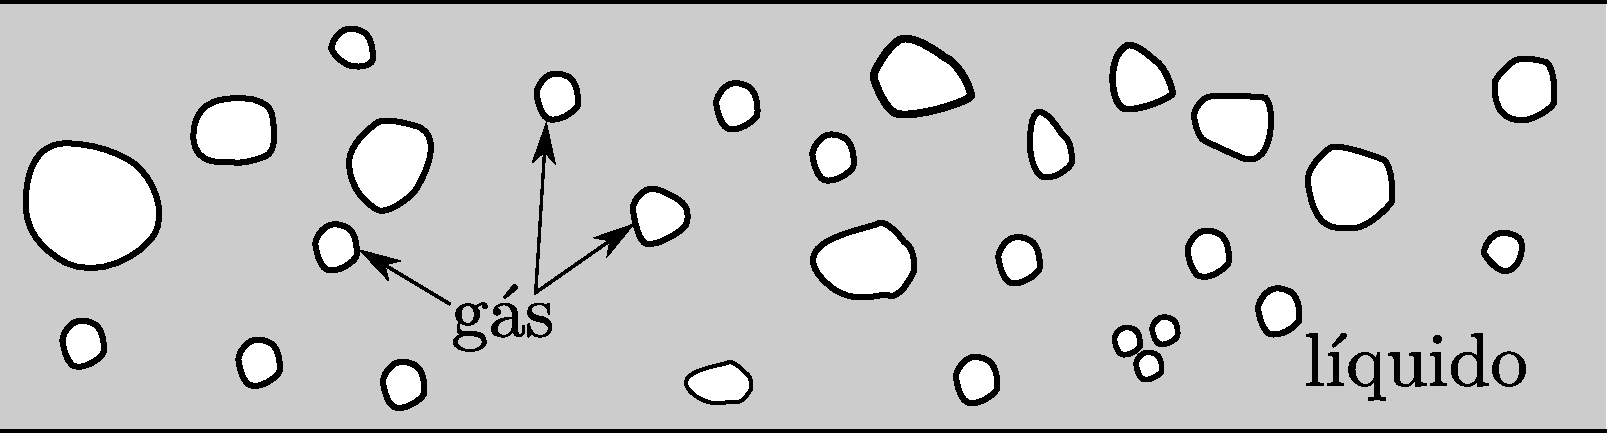
\includegraphics[angle=00, scale=0.3]{h_bubbly.pdf}}\\
		\subfloat[\emph{plug}]
		{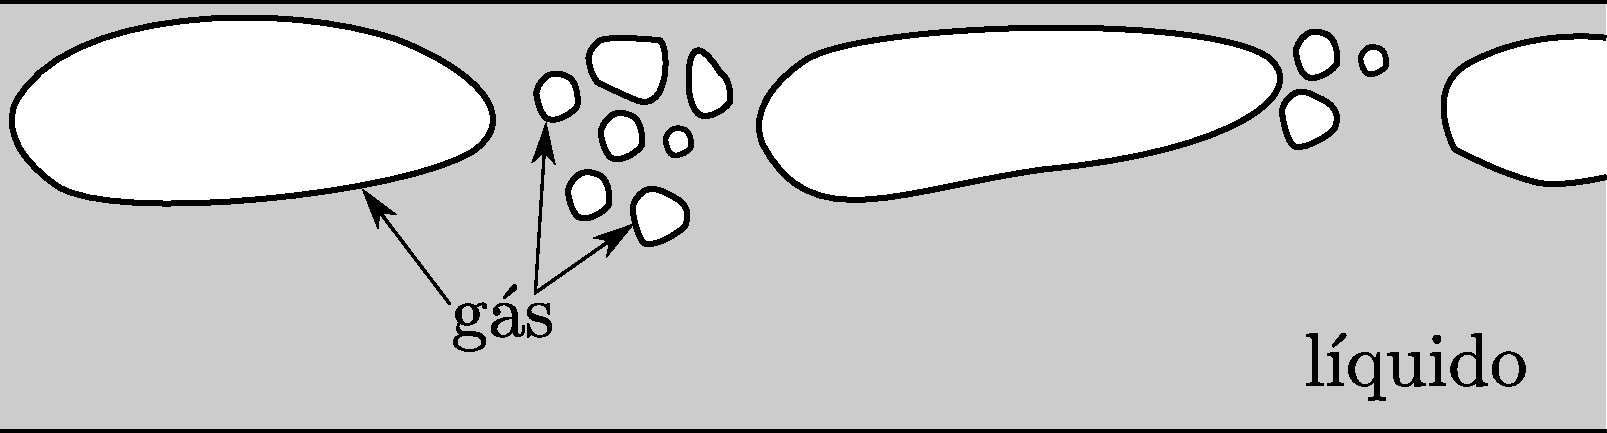
\includegraphics[angle=00, scale=0.3]{h_plug.pdf}}\\
		\subfloat[golfada (\emph{slug})]
		{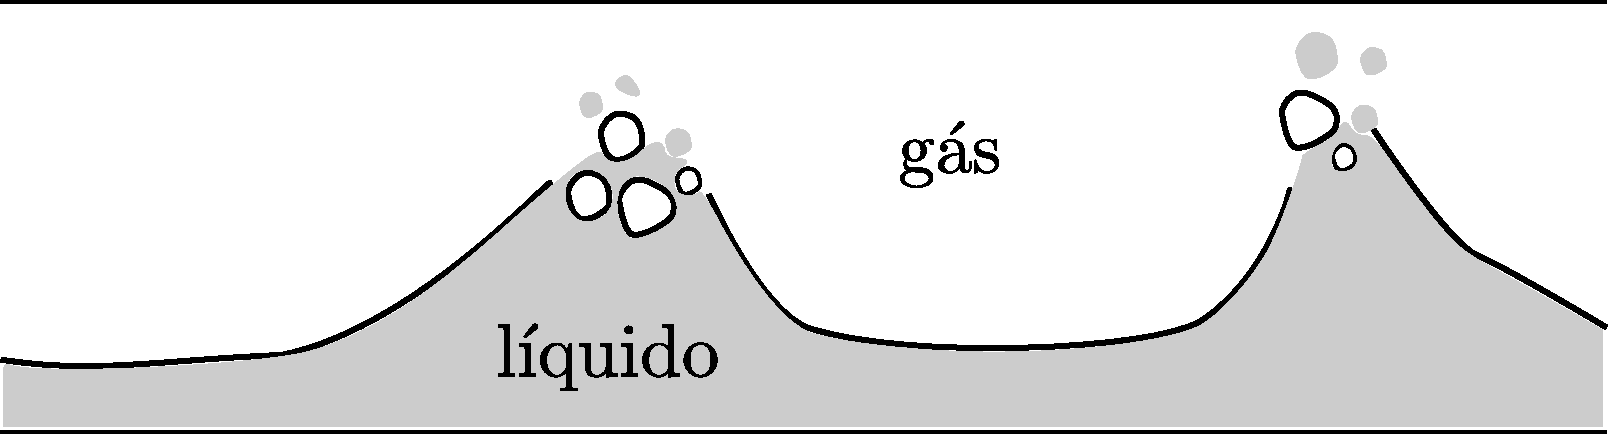
\includegraphics[angle=00, scale=0.3]{h_slug.pdf}}\\
		\subfloat[estratificado (\emph{stratified})]
		{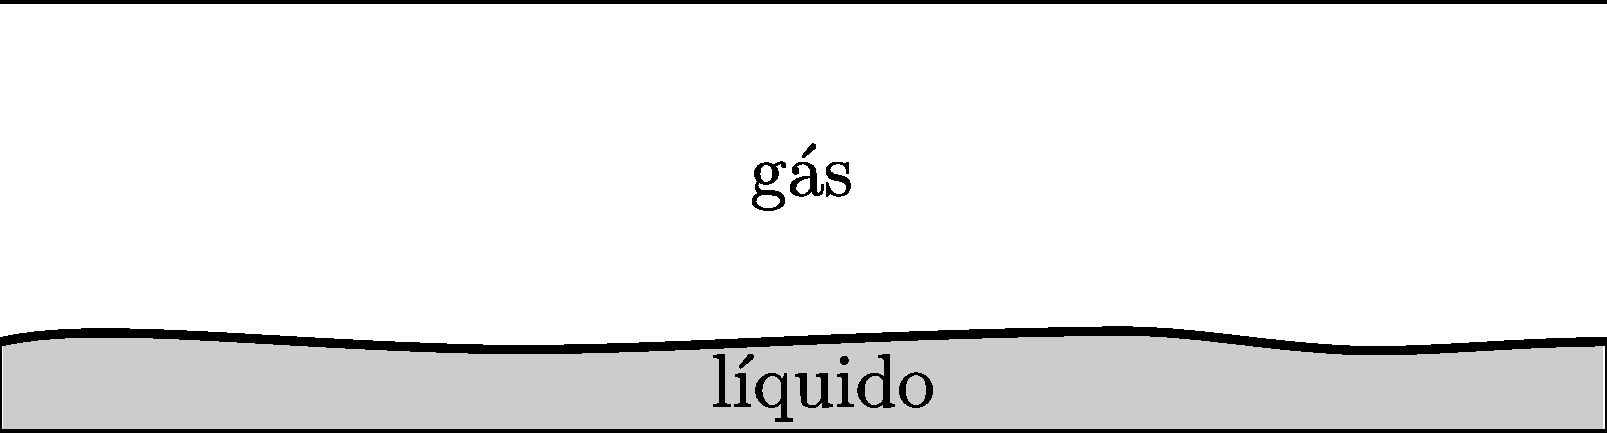
\includegraphics[angle=00, scale=0.3]{h_stratified.pdf}}\\
		\subfloat[ondulado (\emph{wavy})]
		{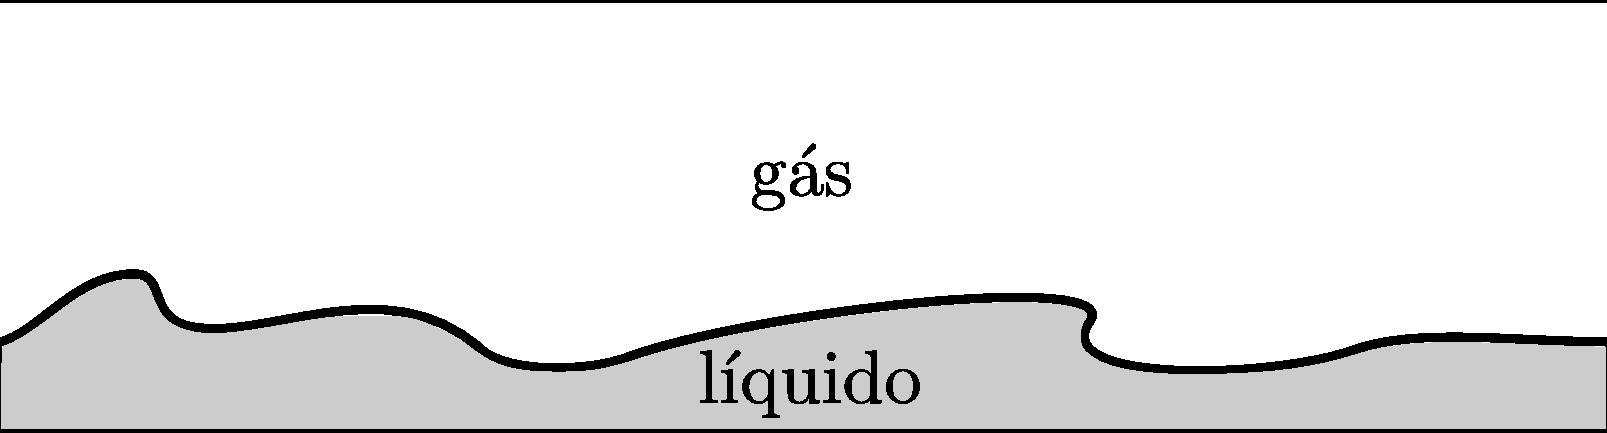
\includegraphics[angle=00, scale=0.3]{h_wavy.pdf}}\\
		\subfloat[anelar (\emph{annular})]
		{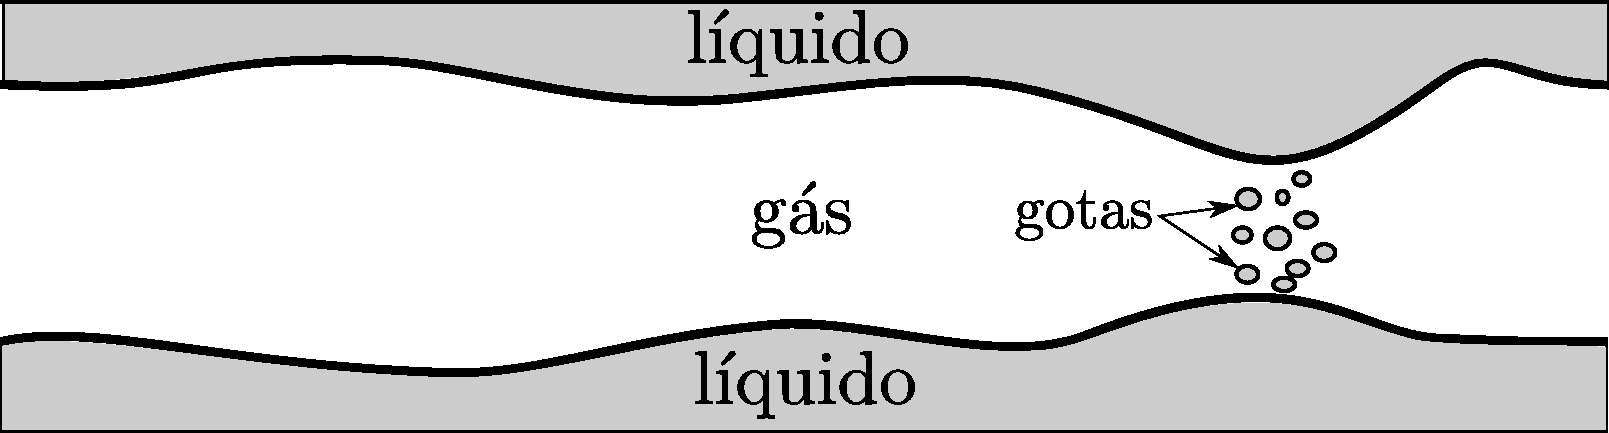
\includegraphics[angle=00, scale=0.3]{h_annular.pdf}}
	\end{center}
	\caption{}
	\label{fig:horizontal} 
\end{figure}

\subsection{Escoamentos verticais}

\begin{figure}[h!]
	\begin{center}
		\subfloat[bolhas (\emph{bubbly})]
		{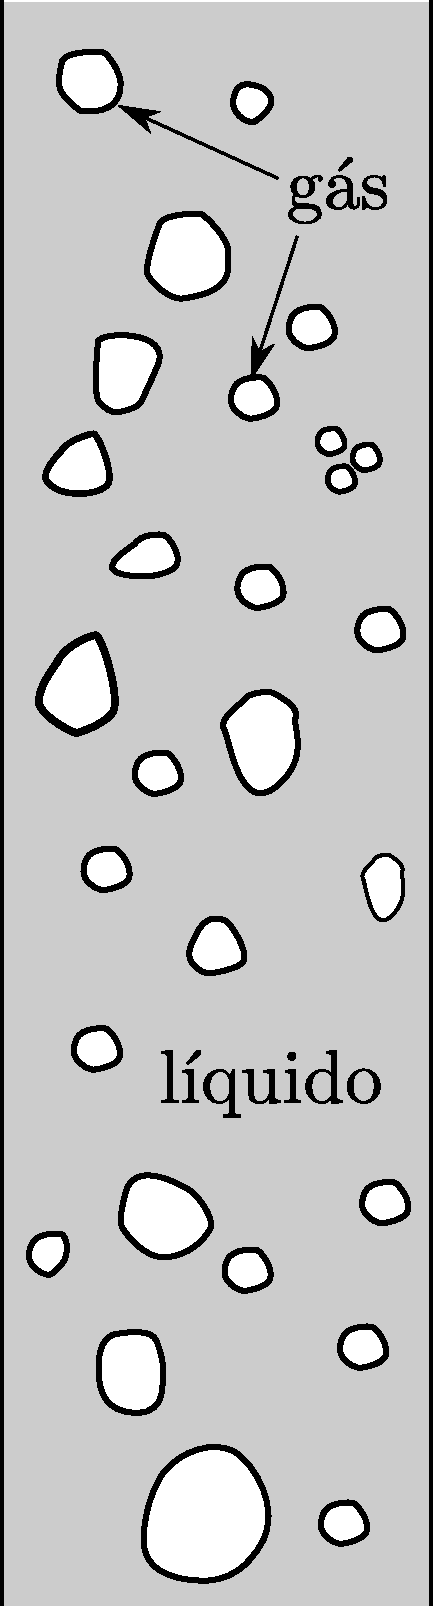
\includegraphics[angle=00, scale=0.3]{v_bubbly.pdf}
		\hspace{0.4cm}}
		\subfloat[golfada (\emph{slug})]
		{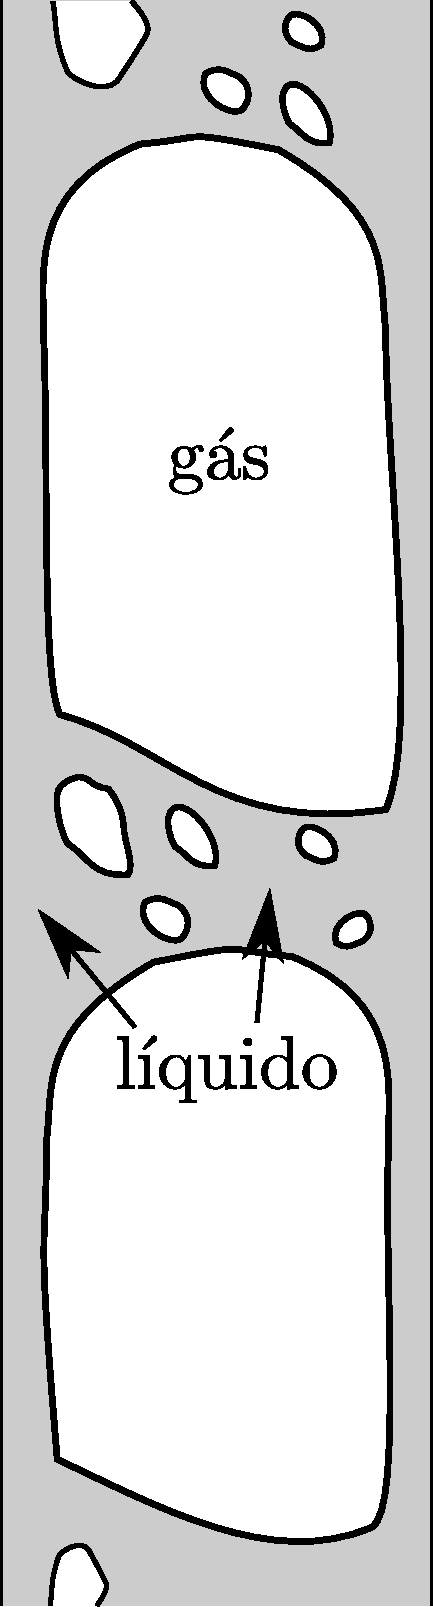
\includegraphics[angle=00, scale=0.3]{v_slug.pdf}
		\hspace{0.4cm}}
		\subfloat[]
		{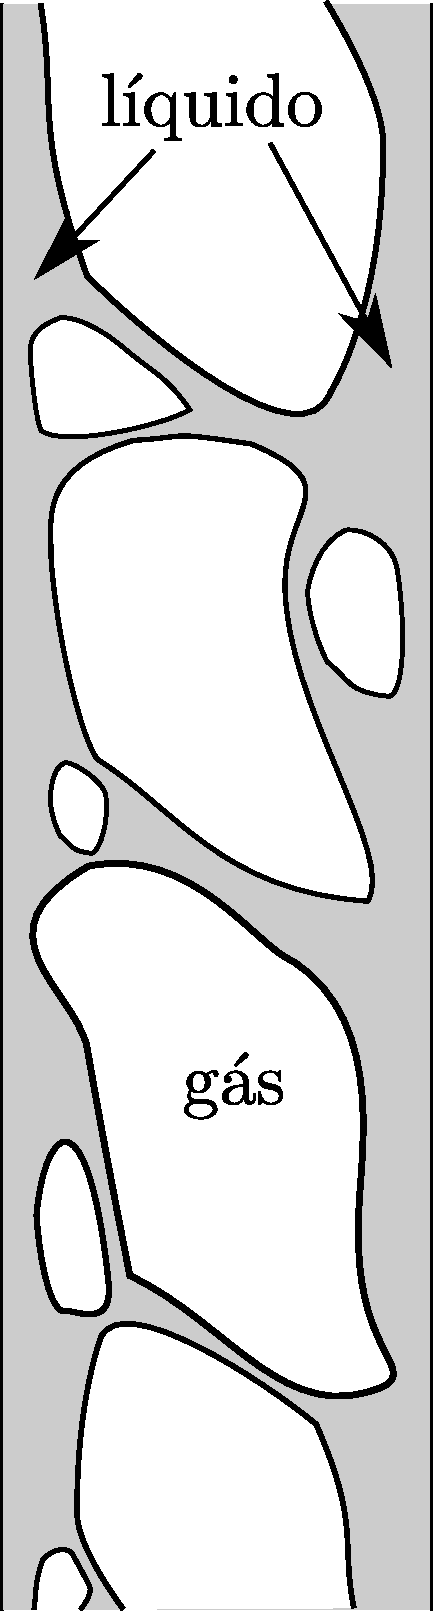
\includegraphics[angle=00, scale=0.3]{v_churn.pdf}
		\hspace{0.4cm}}
		\subfloat[]
		{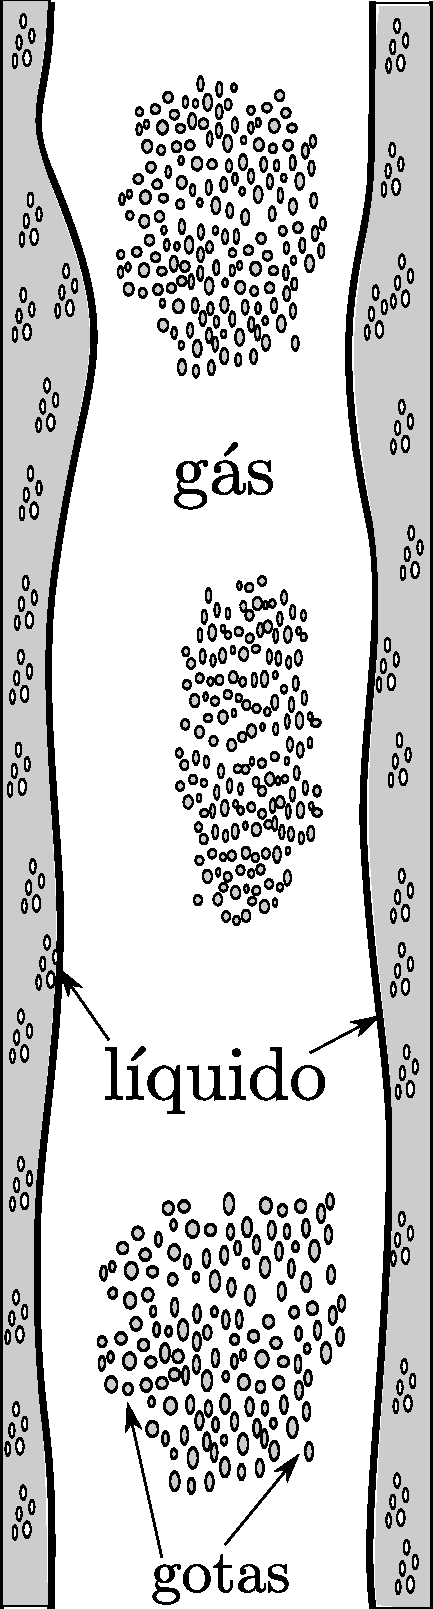
\includegraphics[angle=00, scale=0.3]{v_wispy-annular.pdf}
		\hspace{0.4cm}}
		\subfloat[anelar (\emph{annular})]
		{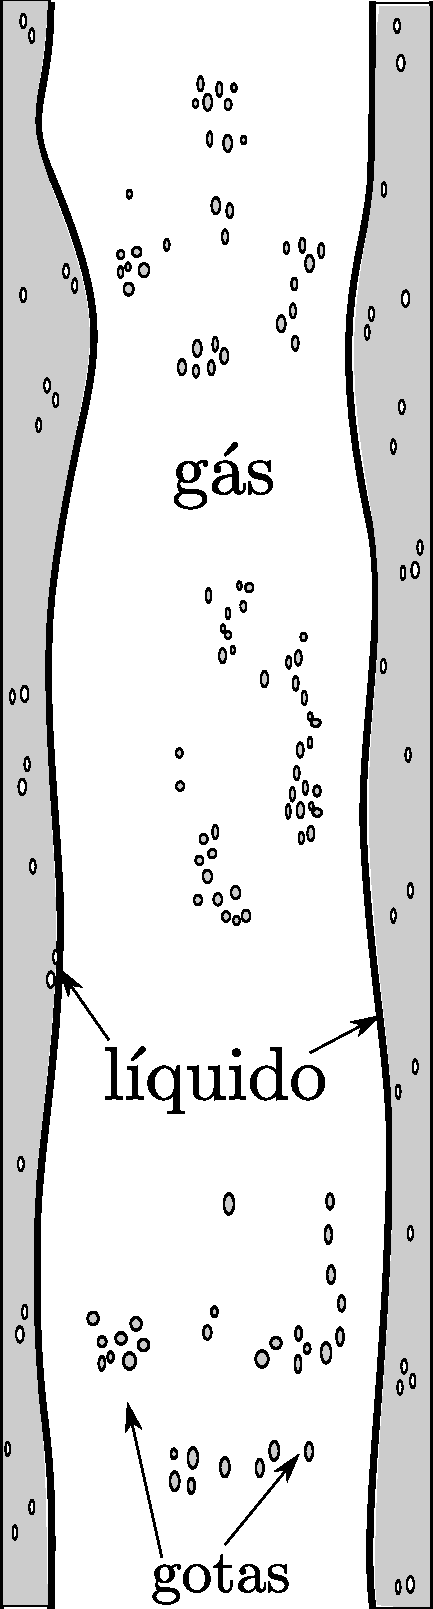
\includegraphics[angle=00, scale=0.3]{v_annular.pdf}}
	\end{center}
	\caption{}
	\label{fig:horizontal} 
\end{figure}

\subsection{Exerc\'icios}

1) Descreva a diferen\c ca entre referencial \emph{Euleriano} e
\emph{Lagrangiano}.


\bibliographystyle{elsarticle-num-names}
\bibliography{$HOME/projects/misc/latex/referencias}

\end{document}

\typeout{ *************** End of file main.tex *************** }
